\section{Problems with the standard model}
\label{sec:problems}
As stated earlier, there are three reasons why the standard model is believed not to provide a full explanation of all natural phenomena. The first pertains to certain observations that seem to directly contradict predictions of the standard model. The second is the behavior seen in some systems that, while not directly contradicting the predictions of the standard model, seem to go beyond the standard model's ability to account for them. And finally, there is the puzzling observation that the standard model contains a high degree of fine tuning.  While the second issue is of much importance, it is not directly relevant to this work, and so further discussion is left to the literature. However, the following is a discussion of the first and last issue.

\subsection{Observations in tension with the standard model}
The most striking shortcoming of the standard model is that it lacks a description for gravity.  Gravity was the first force to be fully understood over large distances, but it will likely be the last to be fully understood at very short distances. This is because the force of gravity is very weak, as it carries a coupling constant that is $10^{34}$ times smaller than the electromagnetic coupling $\alpha$. Gravitational effects would not be observable in particle collisions below a center of mass energy close to the Planck scale ($10^{19}$ GeV), mindbendingly larger than the energetic reach of modern particle colliders. Most theoretical models that could describe the standard model and gravity, sometimes called theories of everything or ultraviolet (UV) completion models, manifest new phenomena only above a large energy called $\cutoff$, roughly in the vicinity of the Planck scale. 

Another observation not predicted by the standard model is that of neutrino mass.  The Higgs field does not interact with neutrinos because neutrinos are left-chiral and have no right-chiral counterparts (see Figure \ref{tab:SM}); neutrinos in the standard model are massless. However, neutrinos were recently observed to oscillate between flavors \cite{Fukuda:1998mi}, a behavior that is only possible if the neutrinos have mass. This seemingly innocuous observation is in fact quite profound, because it implies that some still unknown theory of particles, with masses of higher energy than the standard model, exists. A number of theories have emerged that could potentially explain neutrino mass, including the types I, II, and III seesaw mechanisms \cite{Yanagida:1980xy}, all of which predict heavy right-handed neutrinos whose mass is inversely proportional to the corresponding left-handed neutrino mass. If a lower bound on the masses of the standard model neutrinos were to be measured, this would specify the mass scale of the heavy neutrinos. Unfortunately, no lower bound has been established as yet, and so there are few clues about the nature of the true theory, or at what energy scale the phenomena of the new theory might be observable.

Another piece of evidence that suggests the standard model falls short of providing a full description of nature is the observation of dark matter in galaxies and in the intergalactic regions of the universe \cite{Davis:1985rj}\cite{Komatsu:2008hk}. Measurements of the baryonic mass of galaxies (the mass due to standard model particles) based on observed galactic luminosities are inconsistent with estimates of the total mass of galaxies based on rates of galactic rotation. The baryonic mass is, on average, a factor 6 lower than the total inferred mass, so it seems that there is a great deal of extra mass in galaxies not accounted for by the known particles.  
\begin{figure}[h]
\makebox[\textwidth][c]{
\centering
\subfloat[]{
  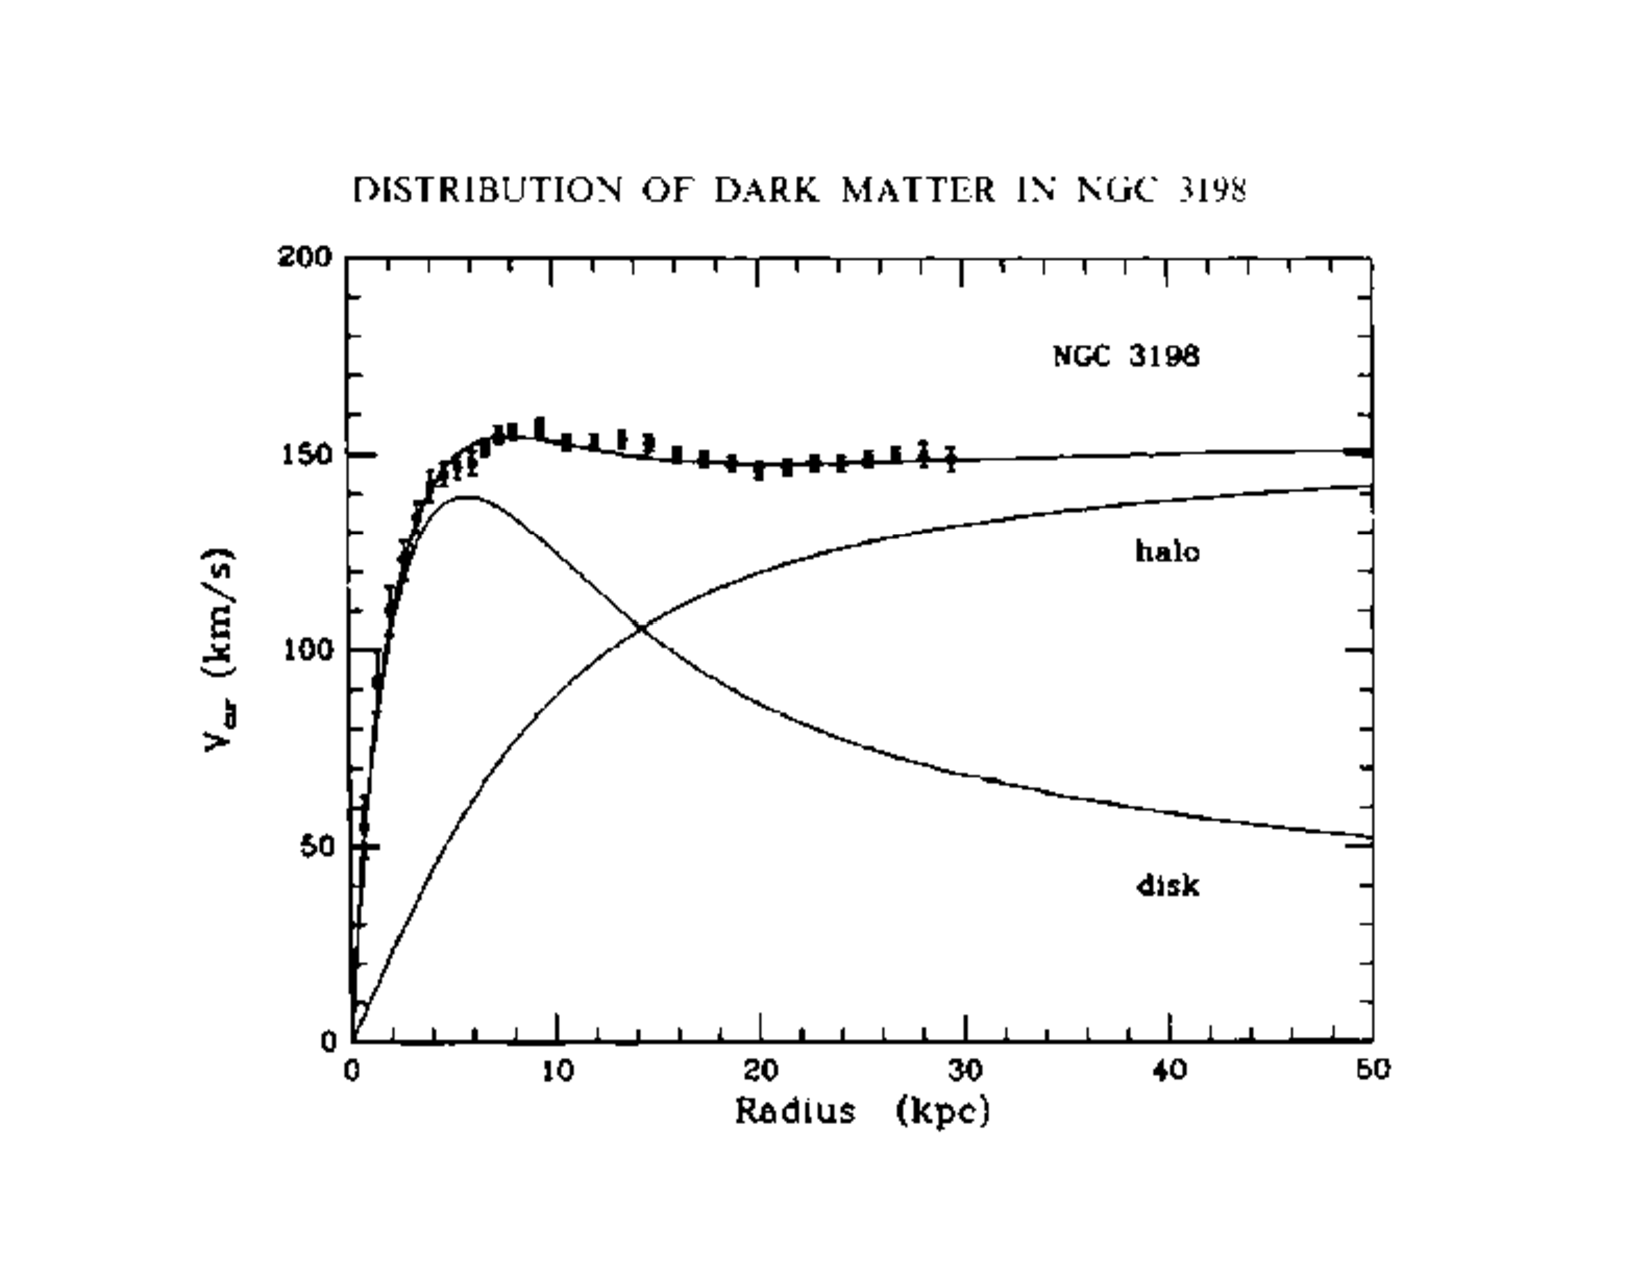
\includegraphics[width=0.6\linewidth]{figures/SM/NGC3198.pdf}
}
\hspace{-.2cm}
\subfloat[]{
  \vspace{2cm}
  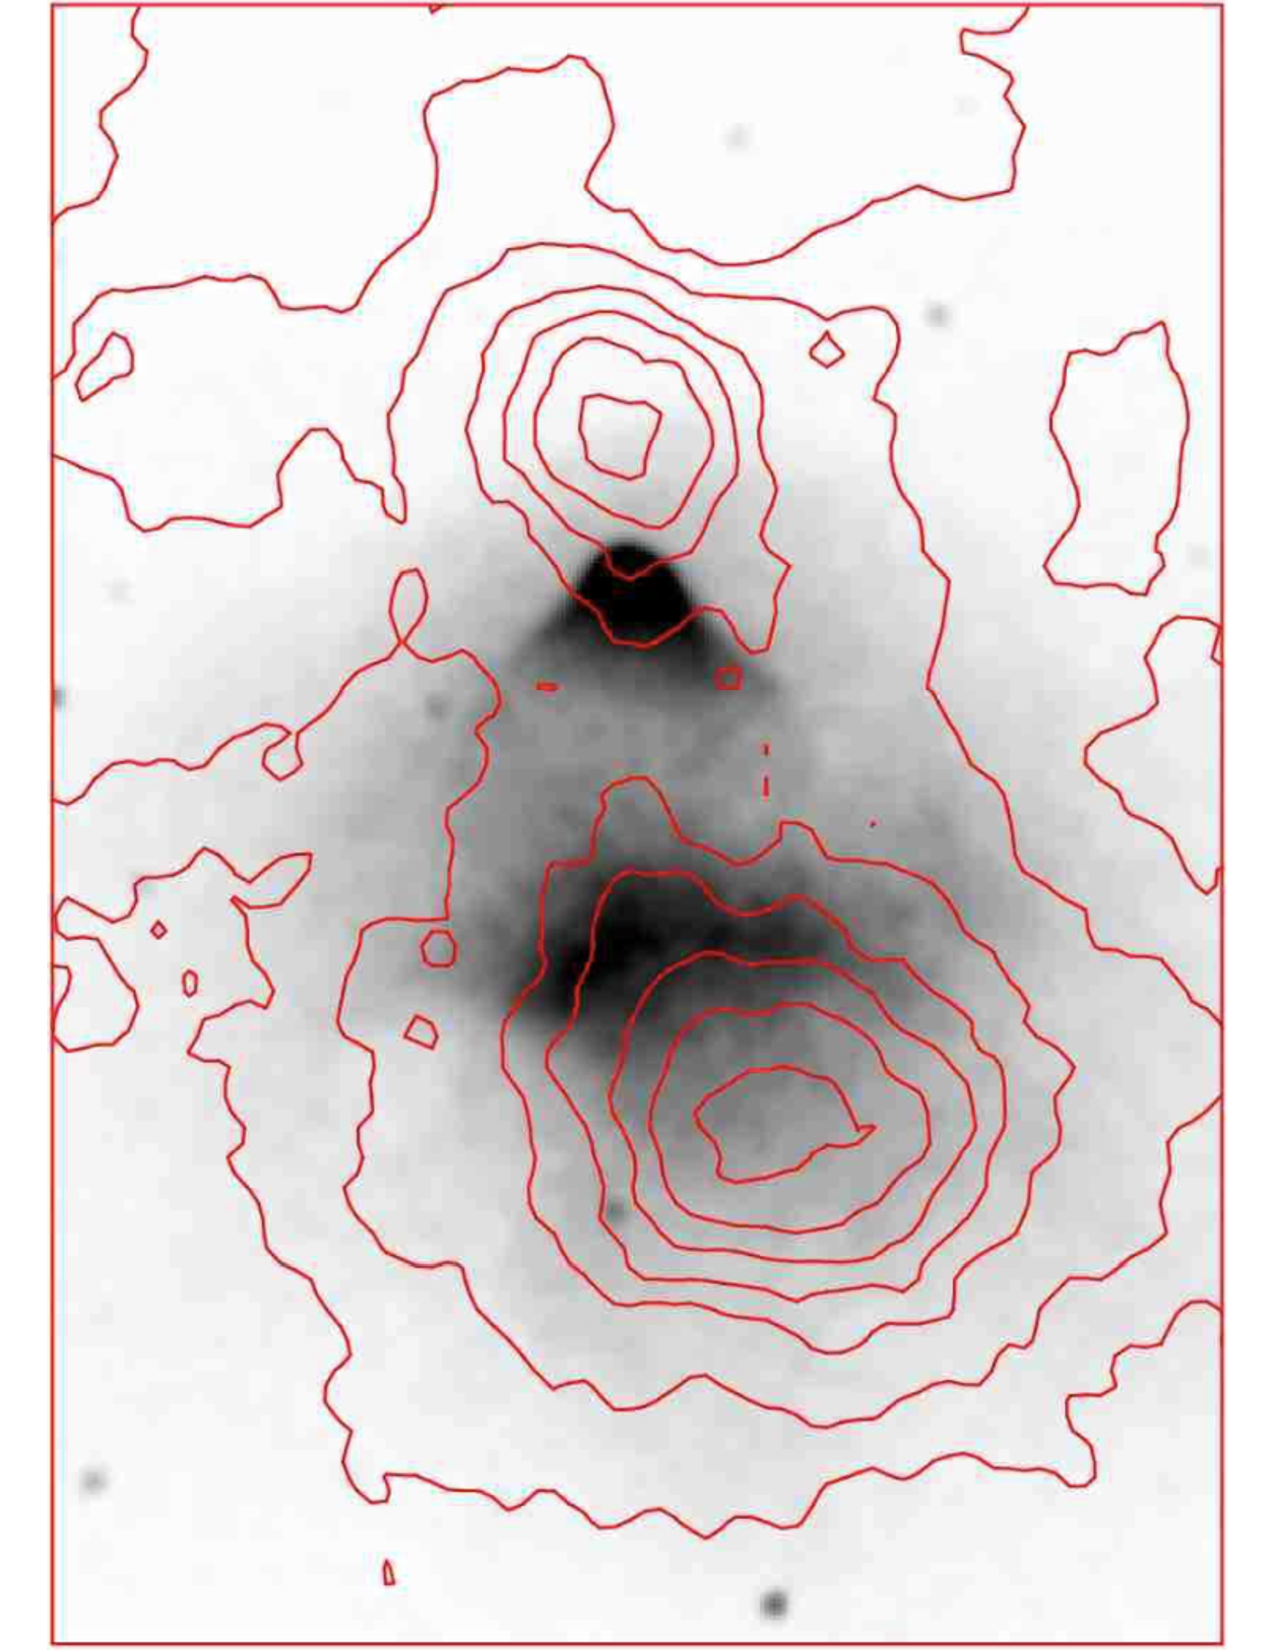
\includegraphics[width=0.46\linewidth]{figures/SM/DMConts.pdf}
}
}
\caption{Subfigure (a) \cite{vanAlbada:1984js} shows the orbital velocity of objects in galaxy NGC 3198 vs their distance from the galactic center. Subfigure (b) \cite{Clowe:2006xq} shows an X-ray photograph taken by the Chandra X-ray observatory of the aftermath of the collision of two galaxy clusters, 1E0657-558, overlaid on a contour map of the gravitation lensing magnitude factor $\kappa$ derived from a separate image taken by the Magellan 6.5 m telescope. } 
\label{fig:DM}
\end{figure}
The best-motivated explanation for this perceived excess is that some yet-undiscovered type of matter exists in abundance within galaxies, but doesn't emit or absorb light (and hence the moniker, ``dark matter''), and therefore has, at most, weak interactions. 

This inferred dark matter may come in the form of new particles, particles not described by the standard model, which may interact with the standard model particles at very high energy scales. This hypothesis is supported by observations of the speed of objects in galaxies as a function of their distance from the galactic center (see Fig. \ref{fig:DM} a). 
The expected speed of objects moving in the nearby galaxy NGC 3198 is given as a function of the orbital radius for the baryonic matter-only hypothesis (solid line peaking at 5 kpc), as well as for the  the baryonic matter+dark matter hypothesis (top solid line). The data (black points) show excellent agreement with the non-interacting dark matter hypothesis. Furthermore, it is claimed that direct evidence of dark matter is evident in the overlay in Figure \ref{fig:DM} (b), in which the aftermath of the collision of two galaxy clusters has been observed. The points of maximum baryonic matter density, represented in black, are displaced from the points of maximum total mass density as determined by the magnitude of gravitational lensing, indicated by the red contours. The interpretation is that the collision of the clusters caused the baryonic matter to collide and slow down, while the dark matter passed through the collision without slowing, resulting in the separation of the two populations of matter.

Dark matter may be discovered by direct or indirect detection experiments (see Ref.~\cite{Undagoitia:2015gya} for a review) or collider experiments like ATLAS \cite{Aad:2008zzm} and CMS \cite{Chatrchyan:2008aa}. A number of theories have been proposed as possible explanations of cosmological dark matter, including certain supersymmetric extensions of the standard model (discussed in Chapter \ref{chap:susy}).


Other observations requiring some explanation beyond the standard model include the fact that there is an abundance of matter in the cosmos but almost no anti-matter (baryon asymmetry), and the existence of the dark energy that accounts for the accelerating expansion of the universe \cite{Goldhaber:2009qu}.

\subsection{Fine tuning and unexplained patterns in the standard model}
\label{sec:finetune}
In a scientific context, tuning is the notion that the parameters of a model can either take on seemingly random values, or they can appear to follow some pattern. An un-tuned (or ``natural'') model refers to the former, and a highly-tuned (or fine-tuned) model refers to the latter. When an apparent pattern has been observed, centuries of science practice and common sense suggests that there should be a reason for the pattern. When a model seems to be fine-tuned, one of two possible, scientifically acceptable explanations must be the case:  
\begin{itemize}
\item{Either there are enough randomized versions (near copies) of the model that the chance emergence of such a pattern is a statistical inevitability; simultaneously, some kind of selection bias has lead the observer to examine the particular instance of the model that exhibited the pattern; or}
\item{there exists some mechanism that generates the observed pattern. }
\end{itemize}
For example, suppose you are shown a piece of toast with the pattern of a religious figure on the face, as in Figure \ref{fig:toast} (a) or (b). 
\begin{figure}[h]
\makebox[\textwidth][c]{
\centering
\subfloat[]{
  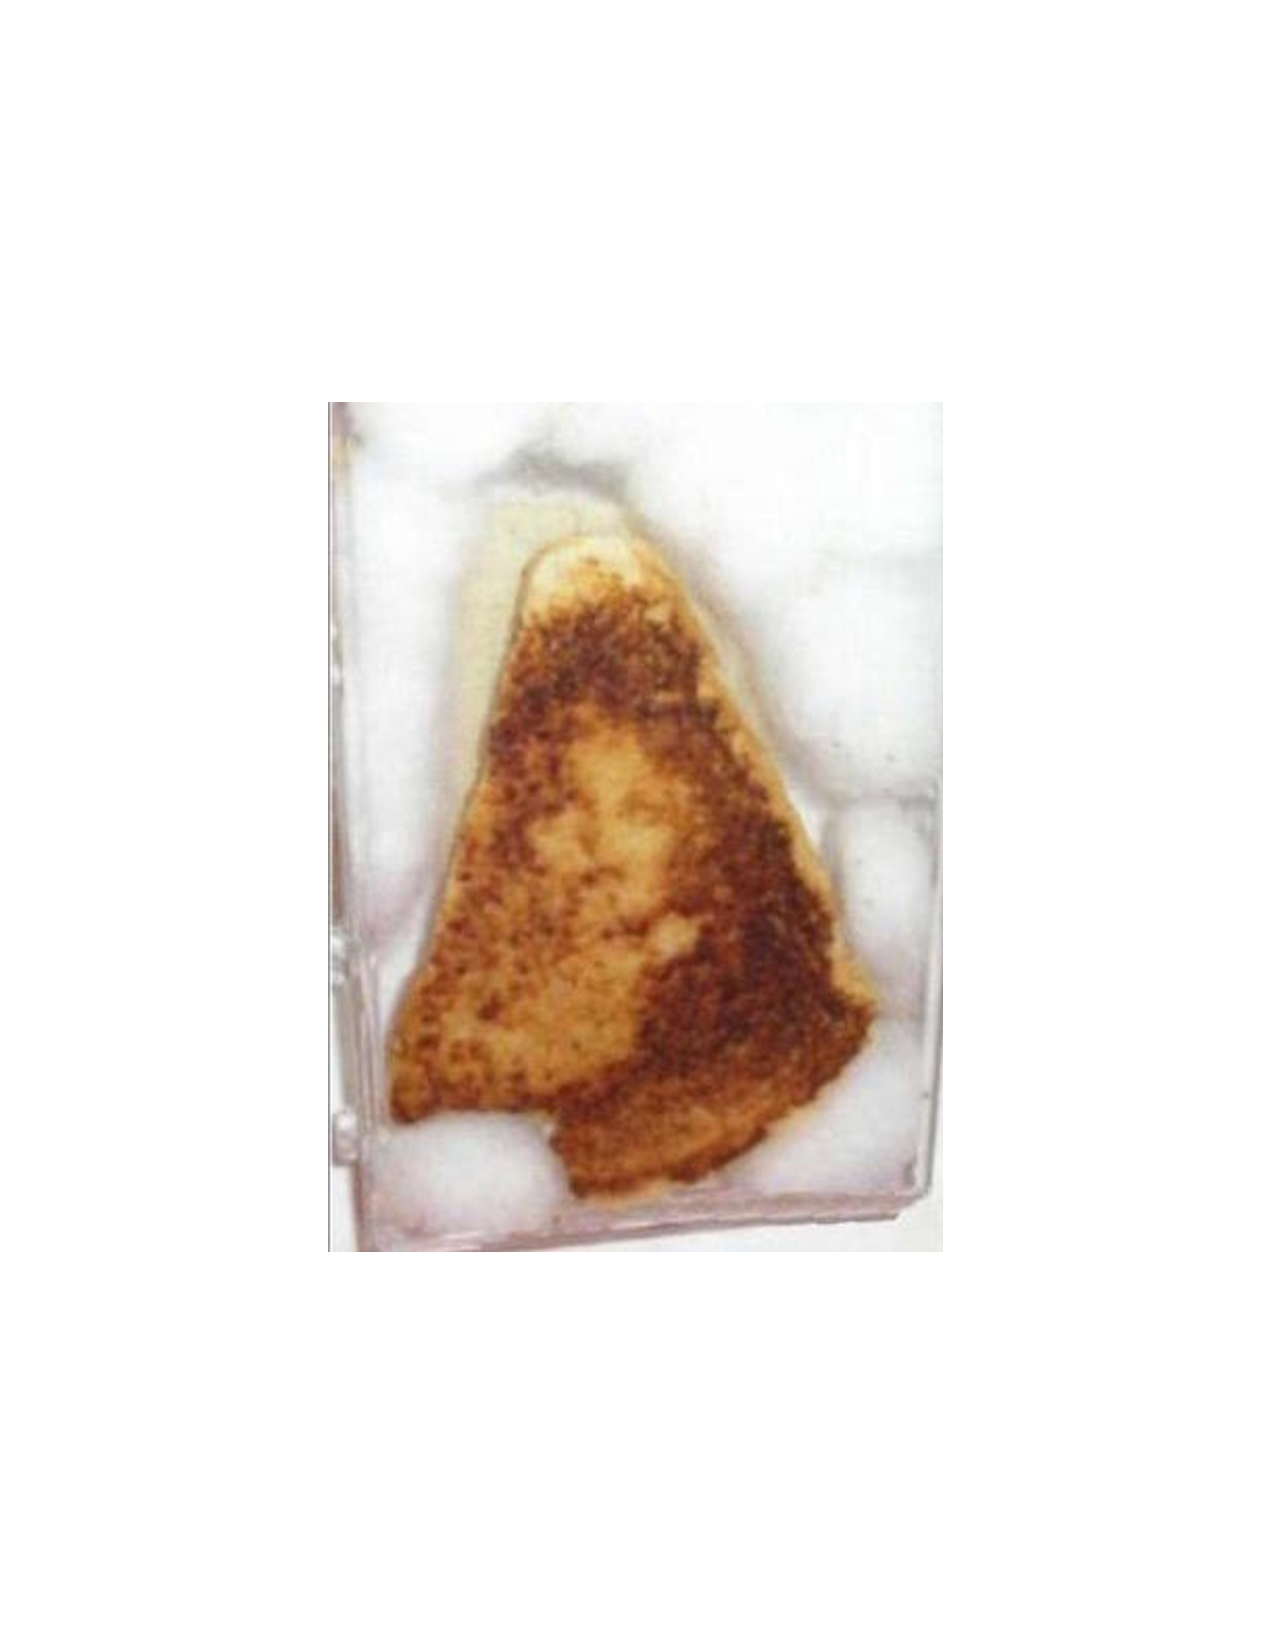
\includegraphics[width=0.3\linewidth]{figures/SM/Mary.pdf}
}
\hspace{-.2cm}
\subfloat[]{
  \vspace{2cm}
  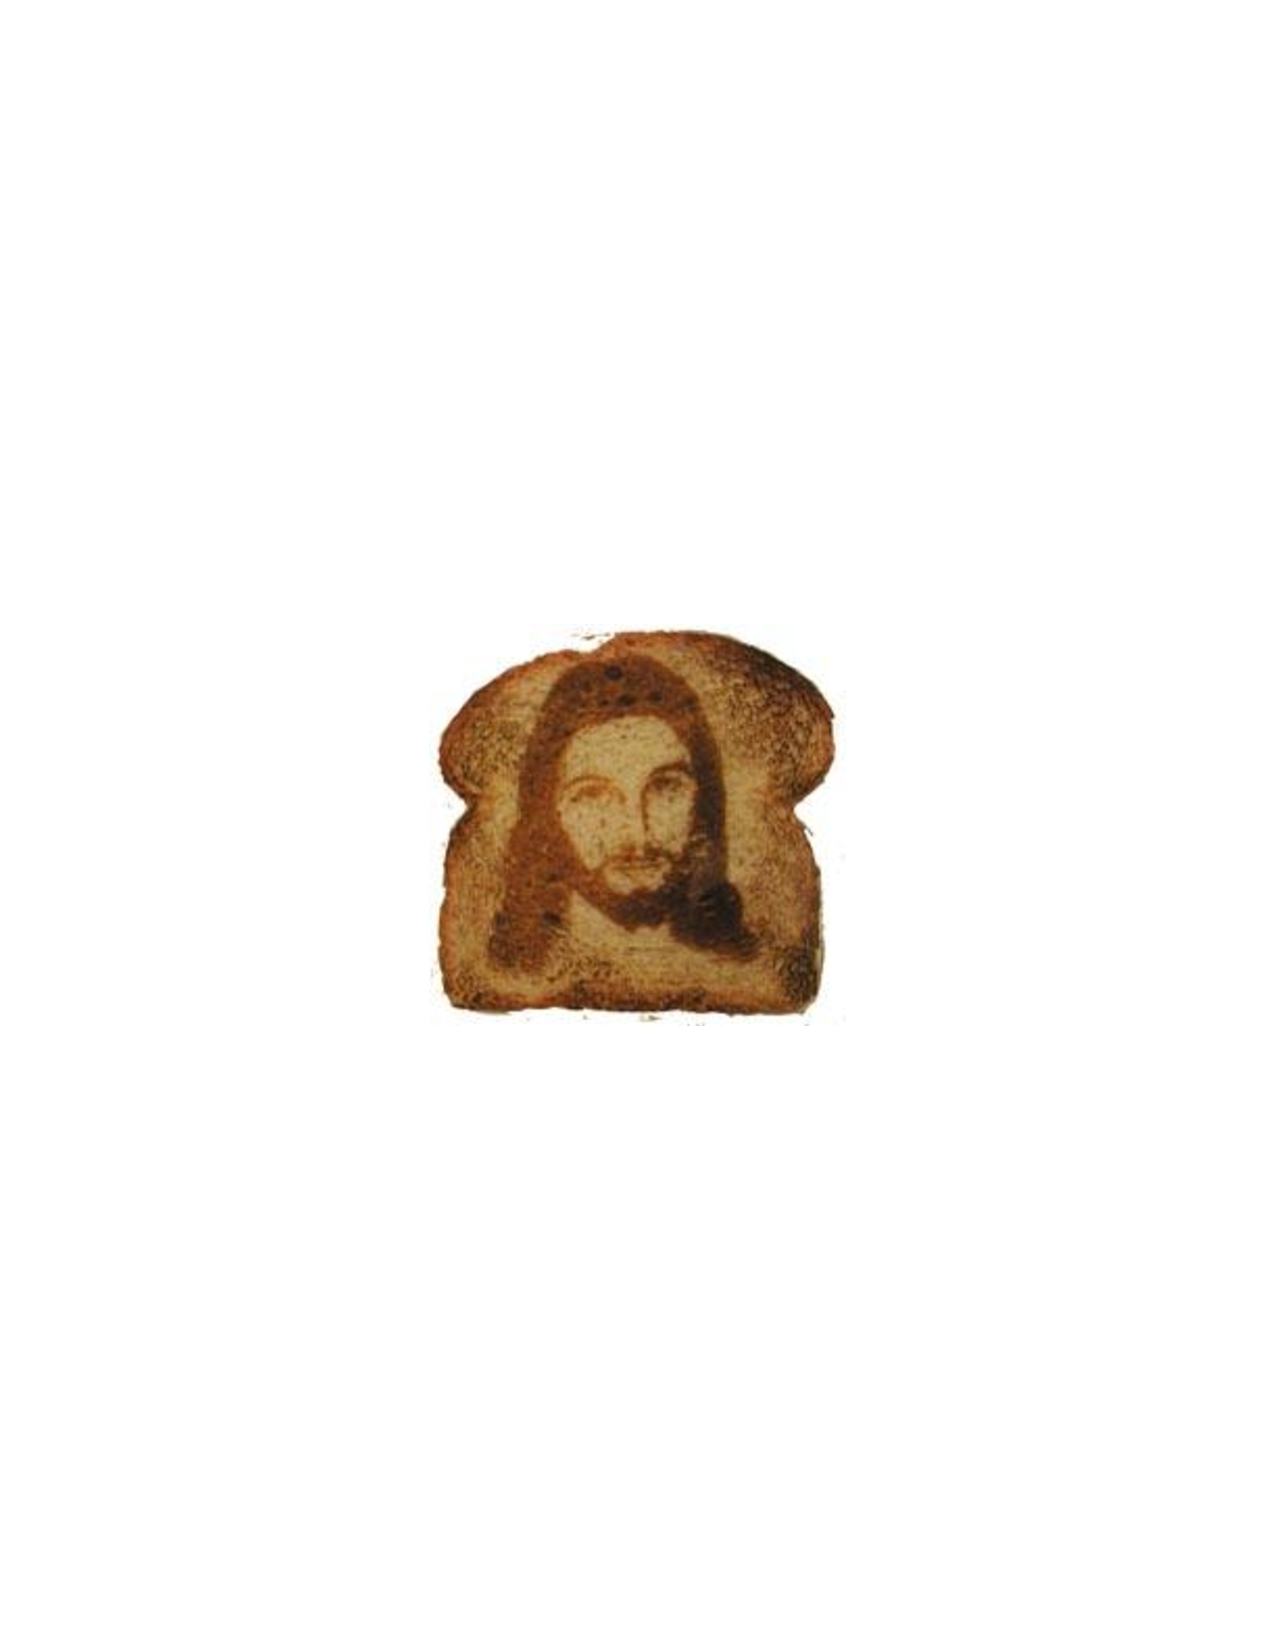
\includegraphics[width=0.33\linewidth]{figures/SM/Jesus.pdf}
}
\hspace{-.2cm}
\subfloat[]{
  \vspace{2cm}
  
\includegraphics[width=0.39\linewidth]{figures/SM/JesusToaster.pdf}
}
}
\caption{[This figure may not be in the final version] Examples of patterns whose reason for emerging is given by each of the scientifically acceptable explanations. } 
\label{fig:toast}
\end{figure}
Both Figs. \ref{fig:toast} (a) and (b) are examples of patterns arising in systems. The scientifically acceptable explanation for the face seen in Fig. \ref{fig:toast} (a) is the first; namely, that enough pieces of toast are made every year that the appearance of such a face on one piece is a statistically inevitability; you see the face in the toast because a selection bias has arisen: the toast some time ago caught the attention of the media, who delivered it to the public consciousness. The pattern seen in Fig. \ref{fig:toast} (b) is justified by the second scientifically acceptable explanation, namely that some mechanism exists, namely, the mechanism featured in Fig. \ref{fig:toast} (c), to bring about the observed pattern.

\begin{figure}[h]
\makebox[\textwidth][c]{
\centering
\subfloat[]{
  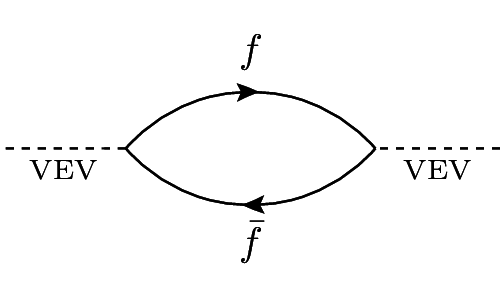
\includegraphics[width=0.5\linewidth]{figures/SM/VevFermionLoop.png}
}
\subfloat[]{
  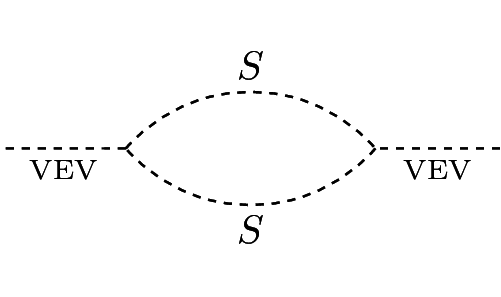
\includegraphics[width=0.5\linewidth]{figures/SM/VevScalarLoop.png}
}
}
\caption{Diagrams for the one-loop corrections to the VEV from a generic fermion (a) and a generic scalar (b).} 
\label{fig:VevLoops}
\end{figure}
The standard model has a number of examples of unexplained fine tuning. Notably, it features a pattern of masses that is quite unusual. As discussed, the origin of particle mass originates from the VEV acquiring a non-zero value through spontaneous symmetry breaking. However, although the VEV is measured to be greater than 200 GeV, it is astonishingly small compared with the natural expectation, and the reason is the following.  The VEV, while normally viewed as a constant in the Lagrangian, actually carries the quantum numbers of the Higgs scalar field, and so interacts with all massive particles. These interactions lead to Feynman diagrams that contain internal loops of the particles. Such diagrams, as in Fig. \ref{fig:VevLoops}, lead to corrections to the value of the VEV given by
\begin{align}
{\rm fermion\hspace{-.1cm}:\ \ }(\Delta {\rm VEV})^2 =& -\frac{\lambda_f^2}{8\pi^2}\cutoff^{2},\label{eq:FermLoop}\\
{\rm scalar\hspace{-.1cm}:\ \ }(\Delta {\rm VEV})^2 =& \hphantom{-} \frac{\lambda_{S}^2}{16\pi^2}[\cutoff^{2}-2m_{S}^2{\rm ln}(\cutoff / m_s)],
\label{eq:ScalarLoop}
\end{align}
where $\lambda_f$ and $\lambda_S$ are the Yukawa coupling and scalar coupling constants, and $\cutoff$ is the cutoff energy of the ultraviolet theory. Every massive particle in the standard model, and in principle any other particle that may occupy the electroweak vacuum, contributes such a correction term. Because $\cutoff$ is near the Planck scale, the VEV receives large corrections that are to $10^{15}$ times larger than the VEV itself. This series of huge numbers is somehow summing to a small number, in a striking example of fine tuning. There is not as yet a scientifically acceptable explanation, since there is no identified mechanism, and no copies of the standard model have been found.

The unexplained cancelation of the 1-loop contributions to the VEV is known as the hierarchy problem, and it impacts nearly every aspect of the standard model. Were the VEV to assume a natural value, the entirety of the particle spectrum of the standard model would be pushed up to the GUT scale. This mystery is especially relevant in the era of TeV-scale particle colliders like the LHC, because a mechanism that could explain the pattern of cancelations is expected to emerge at the electroweak energy scale.  If there is no such mechanism, then we are all but forced to accept the premise that there somehow exists a multitude of versions of the standard model ``somewhere'' in order to make the emergence of such a pattern statistical inevitable. But even in such a case, it is not clear where these copies are, or what selection bias might be responsible for our observing the pattern that is seen. 
